\documentclass[11pt]{article}
\usepackage[letterpaper,margin=1in]{geometry}
\usepackage[T1]{fontenc}
\usepackage[utf8]{inputenc}
\usepackage{lmodern}
\usepackage{amsmath,amssymb,amsthm,mathtools}
\usepackage{booktabs,longtable,tabularx,array}
\usepackage{graphicx}
\usepackage{tikz-cd}
\usepackage{enumitem}
\usepackage{cite}
\usepackage[colorlinks=true,linkcolor=blue,citecolor=blue,urlcolor=blue]{hyperref}

\newtheoremstyle{boldplain}{\topsep}{\topsep}{\itshape}{}{\bfseries}{.}{ }%
  {\thmname{#1}\thmnumber{ #2}\thmnote{ (#3)}}
\newtheoremstyle{boldupright}{\topsep}{\topsep}{\normalfont}{}{\bfseries}{.}{ }%
  {\thmname{#1}\thmnumber{ #2}\thmnote{ (#3)}}
\theoremstyle{boldplain}
\newtheorem{lemma}{Lemma}
\newtheorem{proposition}[lemma]{Proposition}
\theoremstyle{boldupright}
\newtheorem{definition}{Definition}
\newtheorem{example}{Example}

\newcommand{\derived}{[\textup{\textsc{Derived}}]}
\newcommand{\proposed}{[\textup{\textsc{Proposed}}]}
\newcommand{\Dop}{\mathcal{D}}
\newcommand{\cop}{\mathcal{C}}
\newcommand{\Xs}{\mathcal{X}}
\newcommand{\Pc}{\mathcal{P}}
\newcommand{\one}{\mathbf{1}}
\newcommand{\dunk}{d_{\mathrm{unk}}}
\newcommand{\tr}{\operatorname{tr}}
\newcommand{\KL}{\operatorname{KL}}
\newcommand{\Sphys}{S_{\mathrm{phys}}}
\newcommand{\Sadm}{S_{\mathrm{adm}}}

\begin{document}

\begin{center}
  {\LARGE The Identifiability of Color\par}
  \vspace{4pt}
  {\large A Geometric, Relativistic, and Statistical Synthesis of Metameric Projections\par}
  \vspace{18pt}
  {\large Samuel Leizerman\par}
  \vspace{4pt}
  LIOR Research Initiative \quad ORCID: 0009-0000-0133-2291\par
  \vspace{14pt}
  {\large November 2026\par}
\end{center}
\vspace{10pt}

\begin{abstract}
Color is not a property of light. It is a three-dimensional linear readout of a spectral power
distribution, and every readout of that kind identifies infinitely many physically distinct spectra.
We treat this identification, metamerism, as a problem of identifiability: which distinctions a
measurement keeps, which it discards, and which can return. Five results organize the paper.
First, a linear evolution passes to the observed space exactly when it preserves the kernel of the
readout; a relativistic Doppler boost acts on colorimetry as a change of observer, dilating the
color-matching functions, and fails this condition, so metamers separate under motion. Second,
when the evolution does not pass to the observed space, the Mori--Zwanzig projection gives the
observed color an exact memory kernel, and the metameric black enters as the orthogonal term.
Third, Hilbert's projective metric makes the loss precise: the boost is an isometry of the spectral
cone, the colorimetric map is a contraction, and distances in the chromaticity diagram diverge
at the spectral locus, where the set of metamers collapses. Fourth, identifiability under several
measurements is the intersection of their kernels with the tangent structure of the physically
admissible set, a quantity that changes in integer steps; statistical priors, copula dependence,
active perception, and loop closure in robotic mapping are all ways of moving across those steps.
Fifth, when the readouts are local, as with containers over a space of data, identification fails in
two ways: the data may leave directions undetermined, or no global state may reproduce them at
all, and a Farkas inequality certifies the second; one free-energy principle over the consistent set
selects within the undetermined directions and contains maximum entropy, softmax attention,
entropic optimal transport, and Born weights as cases. The components are classical and are
cited as such; what the paper offers is a phrasing in which they are one problem.
Statements are marked \derived{} when they follow from the stated setup and \proposed{}
when they are hypotheses.
\end{abstract}

\section*{Typed symbol table}

{\small
\begin{longtable}{@{}l p{2.7in} p{2.0in} l@{}}
\toprule
Symbol & Meaning & Type & First use\\
\midrule
\endhead
\bottomrule
\endfoot
$\nu,\ \lambda$ & frequency; wavelength & positive reals & \S\ref{sec:intro}\\
$S(\nu)$ & spectral power distribution (spectrum) & nonnegative function & \S\ref{sec:intro}\\
$V$ & space of spectra & real vector space & \S\ref{sec:intro}\\
$K$ & cone of nonnegative spectra & convex cone in $V$ & \S\ref{sec:intro}\\
$\bar x_i$ & color-matching functions, $i=1,2,3$ & nonnegative functions & \S\ref{sec:intro}\\
$C$ & colorimetric readout $S\mapsto(X,Y,Z)$ & linear map $V\to\mathbb{R}^3$ & \S\ref{sec:intro}\\
$\ker C$ & metameric blacks & linear subspace of $V$ & \S\ref{sec:intro}\\
$R$ & Cohen projector onto $\operatorname{span}\{\bar x_i\}$ & orthogonal projector on $V$ & \S\ref{sec:intro}\\
$(x,y)$ & chromaticity coordinates & point of a convex plane region & \S\ref{sec:intro}\\
$u^\mu,\ k^\mu$ & observer four-velocity; photon wave vector & four-vectors & \S\ref{sec:doppler}\\
$\beta,\ \gamma$ & speed over $c$; Lorentz factor & reals & \S\ref{sec:doppler}\\
$D$ & Doppler factor & positive real & \S\ref{sec:doppler}\\
$\eta$ & rapidity, $\beta=\tanh\eta$ & real & \S\ref{sec:doppler}\\
$\Dop_\eta$ & boost acting on spectra & positive linear map $V\to V$ & \S\ref{sec:doppler}\\
$L$ & generator of $\Dop_\eta$ & linear operator on $V$ & \S\ref{sec:doppler}\\
$T,\ \bar T$ & evolution; its quotient on the observed space & maps $V\to V$, $W\to W$ & \S\ref{sec:square}\\
$W$ & observed space, $C(V)$ & vector space & \S\ref{sec:square}\\
$J,\ Z_a,\ e_a$ & carrier $\sum_a Z_a e_a$; amplitudes; quaternion basis & $M_2(\mathbb{C})$; complex; $2\times2$ & \S\ref{sec:square}\\
$\varrho$ & positive closure $JJ^\dagger$ & positive Hermitian $2\times2$ & \S\ref{sec:square}\\
$P,\ Q$ & projector onto resolved variables; $Q=I-P$ & projectors on $V$ & \S\ref{sec:memory}\\
$X=x^\mu\sigma_\mu$ & Hermitian slice element & Hermitian $2\times2$ & \S\ref{sec:hermitian}\\
$\sigma_\mu$ & $(I_2,\sigma_1,\sigma_2,\sigma_3)$, Pauli basis & Hermitian $2\times2$ & \S\ref{sec:hermitian}\\
$B$ & Killing form of $\mathfrak{gl}(2,\mathbb{C})$ & symmetric bilinear form & \S\ref{sec:hermitian}\\
$\Pi$ & effect, $0\le\Pi\le I_2$ & Hermitian $2\times2$ & \S\ref{sec:hermitian}\\
$A,\ U_\gamma$ & connection; holonomy around loop $\gamma$ & Lie-algebra 1-form; group element & \S\ref{sec:hermitian}\\
$\Omega$ & bounded convex domain & subset of $\mathbb{R}^n$ & \S\ref{sec:hilbert}\\
$d_\Omega,\ d_K$ & Hilbert metric on $\Omega$; projective metric on $K$ & metrics & \S\ref{sec:hilbert}\\
$M_i$ & $i$th measurement & linear map $V\to\mathbb{R}^{m_i}$ & \S\ref{sec:hilbert}\\
$\Sphys,\ \Sadm$ & admissible spectra; spectra consistent with data & subsets of $V$ & \S\ref{sec:hilbert}\\
$\mathcal{L}_S$ & lineality space of the tangent cone at $S$ & subspace of $V$ & \S\ref{sec:hilbert}\\
$\dunk$ & dimension of the undetermined space & nonnegative integer & \S\ref{sec:hilbert}\\
$M,\ y$ & stacked measurement $(M_0;\dots;M_n)$; stacked data & linear map; vector & \S\ref{sec:hilbert}\\
$w$ & Farkas certificate & vector of multipliers & \S\ref{sec:hilbert}\\
$\Xs$ & finite data space & finite set & \S\ref{sec:local}\\
$p,\ \Delta(\Xs)$ & distribution on $\Xs$; probability simplex & vector; simplex & \S\ref{sec:local}\\
$U,\ \one_U$ & container; its indicator & subset of $\Xs$; function $\Xs\to\{0,1\}$ & \S\ref{sec:local}\\
$\varphi$ & container coordinates, $\varphi(x)=(\one_{U_k}(x))_k$ & map $\Xs\to\{0,1\}^K$ & \S\ref{sec:local}\\
$\Pc(y)$ & distributions consistent with data $y$ & polytope in $\Delta(\Xs)$ & \S\ref{sec:local}\\
$\Xs_S$ & points charged by some element of $\Pc(y)$ & subset of $\Xs$ & \S\ref{sec:local}\\
$H(p)$ & Shannon entropy, in nats & real & \S\ref{sec:local}\\
$E,\ \tau$ & cost; temperature & function $\Xs\to\mathbb{R}$; positive real & \S\ref{sec:local}\\
$q_\tau$ & Gibbs distribution $e^{-E/\tau}/Z_\tau$ & element of $\Delta(\Xs)$ & \S\ref{sec:local}\\
$\theta$ & multipliers (logits) & vector in $\mathbb{R}^K$ & \S\ref{sec:local}\\
$F_i,\ \cop$ & marginal distribution functions; copula & functions into $[0,1]$ & \S\ref{sec:stat}\\
$\pi$ & pinhole projection & map $\mathbb{R}^3\setminus\{Z=0\}\to\mathbb{R}^2$ & \S\ref{sec:cps}\\
\end{longtable}
}
\addtocounter{table}{-1}

\noindent The script $\cop$ for the copula is distinct from the readout $C$; $D$ is a number and $\Dop_\eta$ an operator.
In \eqref{eq:fracint} $\tau$ is an integration variable; elsewhere it is a temperature. In \eqref{eq:hilbert} $p,q$ are points
of $\Omega$; from \S\ref{sec:local} on, $p$ is a distribution and $q_\tau$ a Gibbs distribution.

\section*{Definitions}

\begin{definition}[Readout]
A readout is a map from a richer structure to a smaller one. It keeps the
distinctions it does not identify and discards the rest. Here the main readout is $C$.
\end{definition}

\begin{definition}[Metamers, metameric black]\label{def:metamer}
Spectra $S_1\neq S_2$ are metamers for $C$ when $C(S_1)=C(S_2)$, that is, when $S_1-S_2\in\ker C$.
An element of $\ker C$ is a metameric black \cite{wyszecki1958,cohen1982}.
\end{definition}

\begin{definition}[Semi-conjugacy, quotient dynamics]
A map $T:V\to V$ passes to the observed space
through $C$ when there is $\bar T:W\to W$ with $C\circ T=\bar T\circ C$. Then $C$ is a semi-conjugacy from $T$ to $\bar T$.
\end{definition}

\begin{definition}[Identifiability]
A state is identifiable from measurements $M_1,\dots,M_n$ on an admissible set when no other admissible state gives the same data. It is locally identifiable when this
holds in a neighborhood \cite{rothenberg1971}.
\end{definition}

\begin{definition}[Positive map, Hilbert metric]
A linear map is positive when it sends the cone $K$
into a cone. The Hilbert metric on a convex domain is the logarithm of a cross-ratio along chords
(\S\ref{sec:hilbert}) \cite{hilbert1895}.
\end{definition}

\begin{definition}[Gluing]\label{def:glue}
Local data on a family of readouts glue when one admissible global state reproduces all of them.
Data that agree wherever two readouts overlap can still fail to glue \cite{abramsky2011}.
\end{definition}

\section{Introduction: the measurement collapse}\label{sec:intro}

A spectral power distribution $S(\nu)$, the power a light carries at each frequency $\nu$, lives in an
infinite-dimensional space $V$. Normal human vision reports three numbers. Grassmann's laws of
color mixture \cite{grassmann1853} and Maxwell's matching experiments \cite{maxwell1860} established that this report is linear, and
the CIE 1931 standard observer \cite{smith1931} fixed it as
\begin{equation}\label{eq:readout}
C(S)=\Bigl(\int S(\nu)\,\bar x_1(\nu)\,d\nu,\ \int S(\nu)\,\bar x_2(\nu)\,d\nu,\ \int S(\nu)\,\bar x_3(\nu)\,d\nu\Bigr)=(X,Y,Z),
\end{equation}
where the nonnegative color-matching functions $\bar x_i$ are the observer. The chromaticity $(x,y)=
(X,Y)/(X+Y+Z)$ discards one more number, overall intensity.

Equation \eqref{eq:readout} has rank three, so its kernel is infinite-dimensional. Wyszecki named the elements
of that kernel metameric blacks \cite{wyszecki1958}: spectra that integrate to zero against every $\bar x_i$ and can be
added to any stimulus without changing its color, within the limits set by nonnegativity. Cohen
and Kappauf gave the decomposition an operator \cite{cohen1982}: with $A$ the matrix whose rows are the $\bar x_i$
on a discretized spectrum, $R=A^{\mathsf T}(AA^{\mathsf T})^{-1}A$ is the orthogonal projector onto the span of the
color-matching functions, and every spectrum splits uniquely as
\begin{equation}\label{eq:cohen}
S=RS+(I-R)S,\qquad C(S)=C(RS),\qquad (I-R)S\in\ker C.
\end{equation}
The fundamental $RS$ carries the color; the residual $(I-R)S$ is invisible. Metamers share a
fundamental and differ in their residuals.

Two consequences follow, and they frame the paper. Color is a readout, not an intrinsic property,
so the question of what a color tells us is a question about which distinctions $C$ keeps. And the
residual is invisible only to this $C$: another observer, another illuminant, or another frame of motion
supplies another readout, and the residual may stop being invisible. Metamerism is therefore an
inverse problem \cite{cohen1982,maloney1986}. A finite set of sensory coordinates cannot reconstruct $S$ without auxiliary
constraints, and the useful questions are which constraints, which additional readouts, and which
dynamics restore the lost distinctions. The thesis of the paper is that the answer has a single
structure seen from five directions: the failure of a semi-conjugacy (\S\ref{sec:square}), the memory kernel it forces
(\S\ref{sec:memory}), the projective geometry that measures it (\S\ref{sec:hermitian}--\S\ref{sec:hilbert}), the local-to-global problem of gluing and
selection (\S\ref{sec:local}), and the statistical and active strategies that
undo it (\S\ref{sec:stat}--\S\ref{sec:cps}).

\section{The Doppler shift as a change of observer}\label{sec:doppler}

The first new readout we consider is motion. A photon with wave vector $k^\mu$ has, for an observer
with four-velocity $u^\mu$, the angular frequency
\begin{equation}\label{eq:omega}
\omega_{\mathrm{obs}}=-k_\mu u^\mu
\end{equation}
in signature $(-,+,+,+)$ \cite{mtw1973}. This is the Doppler shift written invariantly \cite{einstein1905}: it acts on the light
before any physiological filtering. For a source receding or approaching along the line of sight with
speed $\beta c$, frequencies scale by the Doppler factor
\begin{equation}\label{eq:doppler}
D=\sqrt{\tfrac{1+\beta}{1-\beta}}=e^{\eta},\qquad \beta=\tanh\eta,
\end{equation}
with $\beta>0$ for approach; for general direction $D=[\gamma(1-\beta\cos\theta)]^{-1}$.

A frequency shift is not the whole transformation. The photon occupation number is Lorentz
invariant, so specific intensity transforms with $I_\nu/\nu^3$ invariant \cite{rybicki1979}. The boost therefore acts on a
spectrum as
\begin{equation}\label{eq:boost}
(\Dop_\eta S)(\nu)=e^{3\eta}S(e^{-\eta}\nu),\qquad \Dop_{\eta_1}\Dop_{\eta_2}=\Dop_{\eta_1+\eta_2},
\end{equation}
a one-parameter group of positive linear maps with generator $LS=3S-\nu\,\partial_\nu S$. (Per unit wavelength
the same law reads $I_\lambda(\lambda)\mapsto D^5I_\lambda(D\lambda)$.) A blackbody at temperature $T_0$ is carried to a blackbody
at $DT_0$ \cite{peebles1968}, which serves below as a numerical check.

Substituting \eqref{eq:boost} into \eqref{eq:readout} and changing variables $\nu=e^\eta\nu'$,
\begin{equation}\label{eq:dilated}
C_i(\Dop_\eta S)=e^{4\eta}\int S(\nu')\,\bar x_i(e^\eta\nu')\,d\nu'.
\end{equation}
\derived{} A boost of the source is, for colorimetry, a change of observer: the moving observer sees
the original spectrum through dilated color-matching functions $\bar x_i(D\,\cdot)$, rescaled by $D^4$. This places
relativistic metamer breaking in the same class as the familiar failures, change of illuminant and
change of observer \cite{wyszecki1982}, and it is what makes the question of \S\ref{sec:square} sharp.

\section{The broken commutative square}\label{sec:square}

Let $T:V\to V$ be any evolution of the spectrum and $W=C(V)$ the observed space. The observed
color has its own deterministic evolution exactly when the square
\[
\begin{tikzcd}
V \arrow[r,"T"] \arrow[d,"C"'] & V \arrow[d,"C"]\\
W \arrow[r,"\bar T"'] & W
\end{tikzcd}
\]
commutes for some $\bar T$.

\begin{lemma}[Quotient dynamics]\label{lem:quotient}
\derived{} (i) For any surjection $C$ and any map $T$, a map $\bar T$
with $C\circ T=\bar T\circ C$ exists if and only if $C(S_1)=C(S_2)$ implies $C(TS_1)=C(TS_2)$. (ii) If $C$ and $T$
are linear, this holds if and only if $T(\ker C)\subseteq\ker C$, and then $\bar T$ is unique and linear.
\end{lemma}

\begin{proof}
(i) Define $\bar T(w)=C(TS)$ for any $S$ with $C(S)=w$; the implication is exactly well-definedness,
and necessity is immediate from $C(TS_i)=\bar T(C(S_i))$. (ii) For linear maps, $C(S_1)=C(S_2)$ means
$S_1-S_2\in\ker C$, and $C(TS_1)=C(TS_2)$ means $T(S_1-S_2)\in\ker C$.
\end{proof}

Part (i) is the lumpability condition of Kemeny and Snell for Markov chains \cite{kemeny1960}; part (ii) is the
invariant-subspace condition of linear systems theory, where $\ker C$ invariant under the dynamics is
the unobservable subspace \cite{kalman1963,wonham1979}. When the condition fails there are metamers $S_1,S_2$ with
\begin{equation}\label{eq:broken}
C(S_1)=C(S_2)\quad\text{but}\quad C(TS_1)\neq C(TS_2),
\end{equation}
and no deterministic law exists on colors alone.

\begin{proposition}[Metamers separate under boosts]\label{prop:boost}
\derived{} $\Dop_\eta(\ker C)\subseteq\ker C$ if and only if
each dilated function $\bar x_i(e^\eta\,\cdot)$ lies in $\operatorname{span}\{\bar x_1,\bar x_2,\bar x_3\}$.
\end{proposition}

\begin{proof}
By \eqref{eq:dilated}, $\Dop_\eta(\ker C)\subseteq\ker C$ is equivalent to $\ker C\subseteq\ker C_\eta$, where $C_\eta$ has component
functionals $S\mapsto\int S\,\bar x_i(e^\eta\,\cdot)$. For finitely many linear functionals $f_1,f_2,f_3,g$ on a vector space,
$\bigcap_j\ker f_j\subseteq\ker g$ holds if and only if $g\in\operatorname{span}\{f_j\}$, a standard lemma of linear algebra.
\end{proof}

If the color-matching functions were supported in a compact subset of $(0,\infty)$, the condition
could not hold for any $\eta\neq0$: an invariant finite-dimensional span would be invariant under every
power $e^{n\eta}$, whose dilations move any nonzero function's support outside the common support of
the span. Boosts therefore separate metamers. Figure~\ref{fig:boost} shows this with the analytic fit of Wyman,
Sloan, and Shirley to the CIE 1931 functions \cite{wyman2013}. The projection of the dilated functions off the
original span has relative norm 0.11 at $D=1.01$ and 0.47 at $D=1.05$. A pair built as a 5500\,K
blackbody plus a metameric black from \eqref{eq:cohen} matches to machine precision at rest and separates
in chromaticity by $8\times10^{-4}$ at $\beta=0.01$ and $0.028$ at $\beta=0.1$. As a check on \eqref{eq:boost}, the boosted
blackbody reproduces the chromaticity of a blackbody at $DT_0$ to all printed digits.

\begin{figure}[t]
\centering
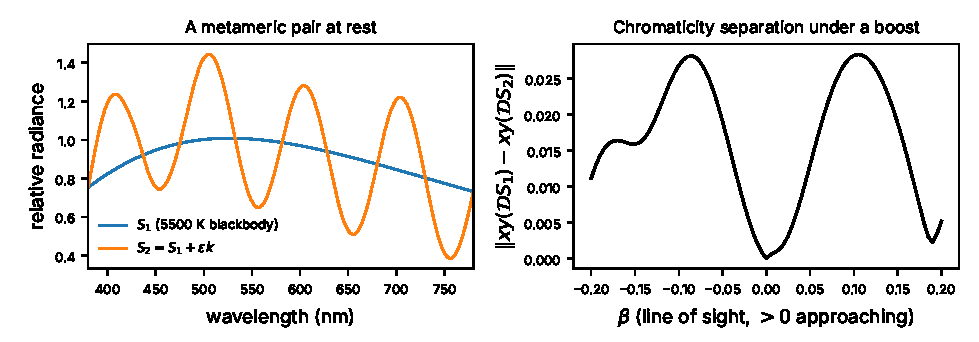
\includegraphics[width=\textwidth]{figure1.pdf}
\caption{Left: a metameric pair, a 5500\,K blackbody $S_1$ and $S_2=S_1+\epsilon k$ with $k=(I-R)g$ a
metameric black. Right: chromaticity separation of the boosted pair as a function of line-of-sight
speed. The separation is zero only at $\beta=0$; it is not monotone because the dilated color-matching
functions sweep across the oscillating black.}
\label{fig:boost}
\end{figure}

The same obstruction appears in matrix form, which \S\ref{sec:hermitian} uses. Assemble four complex amplitudes
$Z_a$ into $J=\sum_{a=0}^3Z_ae_a\in\mathbb{C}\otimes\mathbb{H}\cong M_2(\mathbb{C})$, with $e_0=I_2$ and $e_j=-i\sigma_j$, and read it out by the
positive closure $\varrho=JJ^\dagger$. The readout identifies every $JU$ with $J$ for $U\in U(2)$, and when $\det J\neq0$
the polar decomposition $J=\varrho^{1/2}U$ shows that it identifies nothing else \cite{horn2013}.

\begin{example}[Left and right laws]\label{ex:laws}
\derived{} If $\dot J=\mathcal{L}J$, then $\dot\varrho=\mathcal{L}\varrho+\varrho\mathcal{L}^\dagger$, a law on $\varrho$ alone: the
square commutes. If $\dot J=J\mathcal{R}$, then $\dot\varrho=J(\mathcal{R}+\mathcal{R}^\dagger)J^\dagger=\varrho^{1/2}U(\mathcal{R}+\mathcal{R}^\dagger)U^\dagger\varrho^{1/2}$, which depends on the discarded
unitary $U$ unless the Hermitian part of $\mathcal{R}$ is a multiple of $I_2$. Two carriers with the same closure then have different closures
later: the matrix analogue of \eqref{eq:broken}.
\end{example}

\section{Projection and memory}\label{sec:memory}

When the square does not commute, the observed variable still evolves, but not as a function of its
present value. The Mori--Zwanzig formalism makes this exact \cite{zwanzig1961,mori1965}. For a linear flow $\partial_\eta S=LS$,
a projector $P$ onto the resolved variables, and $Q=I-P$, splitting the flow and solving the $Q$ part
by variation of constants gives
\begin{equation}\label{eq:mz}
\partial_\eta PS(\eta)=PLPS(\eta)+\int_0^\eta PL\,e^{(\eta-s)QLQ}\,QLPS(s)\,ds+PL\,e^{\eta QLQ}\,QS(0).
\end{equation}
The three terms are a Markovian drift, a memory kernel, and a term driven by the initial unresolved
part.

\derived{} Take $P=R$, the Cohen projector of \eqref{eq:cohen}, and $L$ the boost generator of \S\ref{sec:doppler}, so that
$\eta$ is rapidity along a line of sight. Then $PS$ determines $C(S)$ and conversely, and \eqref{eq:mz} is the exact
law of the observed color under a continuously varying boost. The memory kernel vanishes when
$PLQ=0$, which is the infinitesimal form of Lemma~\ref{lem:quotient}: the metameric blacks must not feed the
fundamental. For metamers, $PS_1(0)=PS_2(0)$, so the two observed trajectories differ only through
the last term of \eqref{eq:mz}, the evolved metameric black. The invisible residual is not lost. It is stored in
the orthogonal dynamics and returns through $PLQ$.

This is a general mechanism, not a property of color. Ford, Kac, and Mazur showed that a
Markovian chain of oscillators induces a memory kernel on any single oscillator once the rest are
eliminated \cite{ford1965}; the same holds whenever a readout discards variables that the dynamics couples back.
Two limits of a memory kernel make the present observation sufficient. If the kernel concentrates at
the present, the law forgets; if it retains the whole history without loss, the law is faithful. Every
kernel between them admits no Markov closure on the observed variables. A useful general form for
such kernels is the past-supported fractional integral
\begin{equation}\label{eq:fracint}
(I^\alpha f)(t)=\frac{1}{\Gamma(\alpha)}\int_{-\infty}^t(t-\tau)^{\alpha-1}f(\tau)\,d\tau,
\end{equation}
which interpolates between the identity at $\alpha=0$ and ordinary integration at $\alpha=1$ \cite{samko1993}.

The kernel also has a geometric reading. Path integrals of a 1-form fall into three classes \cite{bott1982}:
exact forms depend only on endpoints; closed forms depend on the topology of the path; non-closed
forms depend on the path through the curvature they enclose. A memory kernel with explicit
dependence on the evaluation time lies outside all three, because extending the history changes the
weight of every earlier segment. Restoring the projected-out variables as a fiber turns the kernel
back into transport, which is the subject of \S\ref{sec:hermitian}.

\section{The Hermitian cone, perceived color, and holonomy}\label{sec:hermitian}

The projection of \S\ref{sec:intro} lands in a cone. Since the $\bar x_i$ are nonnegative, $C$ maps the cone $K$ of nonnegative
spectra into a convex cone in $\mathbb{R}^3$, and Schr\"odinger's axioms make the space of perceived colors
a regular convex cone of dimension at most three \cite{schrodinger1920,provenzi2020}. Resnikoff showed that if this cone is
also homogeneous, there are only two possibilities: the flat cone of Helmholtz--Stiles type, and
$\mathbb{R}^+\times SL(2,\mathbb{R})/SO(2)$, whose chromatic part is the hyperbolic plane \cite{resnikoff1974,provenzi2020}.

The second possibility has a matrix carrier. On the Hermitian slice of $M_2(\mathbb{C})$, write $X=x^\mu\sigma_\mu$
with $\sigma_0=I_2$. Then
\begin{equation}\label{eq:minkowski}
\det X=(x^0)^2-(x^1)^2-(x^2)^2-(x^3)^2,
\end{equation}
the Minkowski form in signature $(+,-,-,-)$; positive semidefinite $X$ form the closed future light
cone, and congruence $X\mapsto GXG^\dagger$ with $G\in SL(2,\mathbb{C})$ preserves \eqref{eq:minkowski} and induces the proper
orthochronous Lorentz group \cite{penrose1984}. The positive closure $\varrho$ of \S\ref{sec:square} lies in this cone, and its trace-one
section $\tfrac12(I_2+\vec r\cdot\vec\sigma)$, $|\vec r|\le1$, is the Bloch ball. Restricting to real symmetric matrices drops $\sigma_2$ and
leaves three real coordinates, a three-dimensional future cone acted on by $SL(2,\mathbb{R})$, whose trace-one
section is a disk.

\derived{} The same algebra also carries a Lie structure and a probability rule, and it is worth stating
exactly how far that goes. The anti-Hermitian part of $M_2(\mathbb{C})$ is $\mathfrak{u}(2)=\mathfrak{su}(2)\oplus\mathfrak{u}(1)$. The Killing
form of $\mathfrak{gl}(2,\mathbb{C})$ is
\begin{equation}\label{eq:killing}
B(\xi,\zeta)=4\tr(\xi\zeta)-2\tr\xi\,\tr\zeta
\end{equation}
\cite{knapp2002}; it vanishes on the central $\mathfrak{u}(1)$ direction and equals $4\tr(\xi\zeta)$ on $\mathfrak{su}(2)$, so the Killing form
of $\mathfrak{u}(2)$ is degenerate, and the trace form agrees with it, up to the factor 4, only on $\mathfrak{su}(2)$. An effect
$\Pi$, $0\le\Pi\le I_2$, assigns to a trace-one state $\hat\varrho$ in the Bloch ball the number $\tr(\hat\varrho\,\Pi)$, which is the Born
rule. Here the algebra supplies the arena but not the law. Gleason's theorem derives the Born rule
from additivity on projections only in dimension three or more \cite{gleason1957}; in dimension two the derivation
holds for additive measures on effects \cite{busch2003}, which is an additional assumption about what a measurement
is. One carrier holding the Lorentz form \eqref{eq:minkowski}, the Bloch ball, the Killing form \eqref{eq:killing}, and Born weights
is therefore a statement about where these structures live, not a derivation of any of them; what a
dynamics on the carrier would impose across them is the content of open question~1 in \S\ref{sec:synth}.

Berthier identified this real slice with perceived color \cite{berthier2020}: the space of perceived colors is the
effect space of a rebit, a two-level real quantum system, whose chromatic state space is the Bloch
disk. The disk coincides with Hering's opponent disk, its two chromatic coordinates playing the
roles of the two opponent axes, and its natural metric is Klein's, which is Hilbert's metric on the
disk (\S\ref{sec:hilbert}). Berthier, Garcin, Prencipe, and Provenzi then derived relativistic properties of perceived
color, of the kind Yilmaz argued for experimentally \cite{yilmaz1962}, from this model and a single trichromacy
axiom \cite{berthier2021}. On this route the Lorentzian structure of color is citable, and it lives on the same carrier
as \eqref{eq:minkowski}.

\derived{} Transport on this carrier has holonomy. Let $A$ be a connection with values in the
Lie algebra of the structure group; transport around a loop $\gamma$ is the path-ordered exponential
\begin{equation}\label{eq:holonomy}
U_\gamma=\mathcal{P}\exp\Bigl(-\oint_\gamma A\Bigr),
\end{equation}
which changes by conjugation under a gauge transformation, so its trace, the Wilson loop, is gauge
invariant \cite{kobayashi1963,wu1975}. For the hyperbolic disk, with curvature $-1$, Levi-Civita transport around a
geodesic triangle rotates tangent vectors by the angular defect $\pi-(\alpha+\beta+\gamma)$, which by Gauss--Bonnet
equals the enclosed area \cite{docarmo1976}. In group terms, the composition of two non-collinear boosts is a boost
followed by a rotation, the Thomas--Wigner rotation \cite{thomas1926,wigner1939}, and that rotation is this holonomy.

\proposed{} If changes of viewing condition act on chromatic states as $SL(2,\mathbb{R})$ transformations
of the disk, the group that acts on the rebit state cone, then a sequence of such changes that returns
to its starting condition leaves a residual rotation of the chromatic disk, a hue rotation, equal to the
hyperbolic area the sequence encloses. A loop of adaptation would then leave a trace that depends
on its shape, not on its duration. This is a test: present closed loops of background change and
measure the residual hue shift against the enclosed area.

The physical boost of \S\ref{sec:doppler} and the perceptual transformations of this section are different group
actions on different spaces: one on spectra before the readout, one on perceived states after it.
Whether a principled relation exists between them is open, and \S\ref{sec:synth} returns to it.

\section{Hilbert geometry and the identifiability frontier}\label{sec:hilbert}

The previous sections located the loss; this one measures it. For a bounded convex domain $\Omega$ and
distinct $p,q\in\Omega$, let the line through them meet $\partial\Omega$ at $a$ and $b$, in the order $a,p,q,b$. Hilbert's
metric is \cite{hilbert1895}
\begin{equation}\label{eq:hilbert}
d_\Omega(p,q)=\tfrac12\log\frac{|p-b|\,|q-a|}{|p-a|\,|q-b|}.
\end{equation}
On the disk it is the Klein model of the hyperbolic plane, and it is invariant under projective
maps of $\Omega$ because it is a cross-ratio. On a closed cone $K$, with $M(f/g)=\inf\{t:f\le tg\}$ and
$m(f/g)=\sup\{t:f\ge tg\}$, the projective version is
\begin{equation}\label{eq:projmetric}
d_K(f,g)=\log\frac{M(f/g)}{m(f/g)},
\end{equation}
which for nonnegative spectra is $\log\bigl[\sup(f/g)\,\sup(g/f)\bigr]$ and vanishes exactly on rays \cite{birkhoff1957,bushell1973}.

\begin{proposition}[Where distinguishability is lost]\label{prop:hilbert}
\derived{} (i) Each boost $\Dop_\eta$ is an isometry of
$d_K$ on the cone of spectra. (ii) The readout $C$ does not expand Hilbert distances: $d_{C(K)}(Cf,Cg)\le
d_K(f,g)$, with Birkhoff--Hopf contraction ratio $\tanh(\Delta/4)$ when the image has finite projective
diameter $\Delta$. (iii) For metamers, $d_K(S_1,S_2)>0$ while $d_{C(K)}(CS_1,CS_2)=0$.
\end{proposition}

\begin{proof}
(i) $\Dop_\eta$ is positive with positive inverse $\Dop_{-\eta}$, so $f\le tg$ if and only if $\Dop_\eta f\le t\,\Dop_\eta g$; hence $M$
and $m$ are unchanged. (ii) $f\le tg$ implies $Cf\le tCg$ in the image cone, so $M$ cannot increase and
$m$ cannot decrease; the ratio is Birkhoff's theorem \cite{birkhoff1957}, extended by Hopf \cite{hopf1963} and Bushell \cite{bushell1973}. (iii)
Metamers are distinct rays with equal images.
\end{proof}

The proposition separates three things that are easy to conflate. Motion does not destroy
spectral distinguishability: for the pair of Figure~\ref{fig:boost}, $d_K=1.0667$ at rest and $1.0666$ at $\beta=0.1$ and
$0.2$, equal up to discretization. The readout $C$ is where distinctions are lost, and a boost changes
which ones by changing the effective observer. Because \eqref{eq:hilbert} is a cross-ratio, the projective metric
on the image cone equals twice Hilbert's metric \eqref{eq:hilbert} on any affine section, and so on the chromaticity diagram,
whose closure is convex: the convex hull of the spectral locus and the purple line \cite{wyszecki1982}.

The boundary carries the identifiability content. As $q$ approaches the spectral locus, \eqref{eq:hilbert} diverges,
so small changes in measurement near saturated colors are large changes in distinguishability. The
metamer set behaves the same way: on the strictly convex part of the locus, the only lights with
a given chromaticity are monochromatic at one wavelength, so the admissible fiber collapses to a
ray. Stiles and Wyszecki found that the number of metameric object colors peaks at the achromatic
point and falls toward saturation \cite{stiles1962}. \proposed{} The size of the admissible fiber $C^{-1}(y)\cap K$ is a
decreasing function of the Hilbert distance from $y$ to the white point; the divergence of $d_\Omega$ at the
locus and the collapse of the metamer set are the same phenomenon seen from the image and from
the fiber.

\paragraph{Several measurements.} Let $M_0,\dots,M_n$ be linear measurements, for instance $C$ under different
illuminants or observers. Data $y_i$ restrict the spectrum to
\begin{equation}\label{eq:adm}
\Sadm=\bigcap_{i=0}^nM_i^{-1}(y_i)\cap\Sphys,\qquad
\ker\begin{pmatrix}M_0\\ \vdots\\ M_n\end{pmatrix}=\bigcap_{i=0}^n\ker M_i,
\end{equation}
where $\Sphys$ encodes nonnegativity, normalization, and band limits. At a point $S$ of $\Sphys=K$ that
vanishes on a set $Z$, the admissible directions form the cone $\{\delta S\ge0\text{ on }Z\}$, whose largest subspace
is the lineality space $\mathcal{L}_S=\{\delta S=0\text{ on }Z\}$. Define
\begin{equation}\label{eq:dunk}
\dunk(S)=\dim\Bigl(\bigcap_{i=0}^n\ker M_i\cap\mathcal{L}_S\Bigr).
\end{equation}
\derived{} In a finite discretization, $\dunk$ is an integer that cannot increase when a measurement
is added, decreases by the number of independent new constraints, and drops when $S$ moves onto
a face of the cone. At a regular point, local identifiability holds exactly when $\dunk=0$, which
is Rothenberg's rank condition \cite{rothenberg1971} written for linear readouts. The identifiability frontier is the
set of conditions at which $\dunk$ steps. Because the lineality space is used, $\dunk$ counts directions
undetermined in both senses; one-sided directions at the boundary are constrained by inequality,
which is where the Hilbert divergence above enters.

\paragraph{Inconsistency.} $\dunk$ measures one way identification fails: too many spectra fit the data. The
other is that none does. Measurements taken separately, under different illuminants, by different
observers, or with noise, can leave $\Sadm$ in \eqref{eq:adm} empty. Write $M$ for the stacked measurement in
\eqref{eq:adm} and $y$ for the stacked data, with normalization and band limits included as rows, so that $\Sphys=K$.
\derived{} In a finite discretization $K$ is a polyhedral cone and \eqref{eq:adm} is a linear feasibility problem, so
Farkas' lemma \cite{farkas1902} gives an exact alternative: either $\Sadm\neq\emptyset$, or there is a vector $w$ with
\begin{equation}\label{eq:farkas}
\langle w,MS\rangle\ge0\ \text{ for every }S\in K\qquad\text{and}\qquad\langle w,y\rangle<0.
\end{equation}
The second alternative is an inequality on data alone, satisfied by everything a physical spectrum can
produce and violated by $y$, and it can be checked without reconstructing $S$. For a single readout it is a
supporting hyperplane of the image cone $C(K)$: a reported color whose chromaticity lies outside the
spectral locus and purple line is certified inconsistent by a line that separates it from the diagram. With
several readouts the condition is stronger than each one separately: every $y_i$ can lie in its own image
cone $M_i(K)$ while the stacked $y$ lies outside $M(K)$. That is a failure to glue in the sense of
Definition~\ref{def:glue}, and \S\ref{sec:local} treats it directly. Identifiability therefore has two frontiers: $\dunk$ steps on one side,
and on the other the consistent set empties. Near the spectral locus, where the fiber is already small,
little noise is needed to cross from the first to the second.

\section{Local readouts: gluing, identifiability, and selection}\label{sec:local}

The same structure answers a question that arises whenever data come in pieces: given a space of
data and a set of containers over it, how should the data be modeled? Every ingredient below is
classical: Farkas' lemma \cite{farkas1902}, Jaynes' maximum entropy \cite{jaynes1957}, Csisz\'ar's I-projection \cite{csiszar1975},
Vorob'ev's extension theorem \cite{vorobev1962}, and Sinkhorn scaling \cite{sinkhorn1964,cuturi2013}. What this section adds is a
phrasing in which the container question and the identifiability problem of \S\ref{sec:hilbert} are one problem, so
that gluing, identifiability, and selection become three questions about a single linear readout.

\paragraph{Containers as readouts.} Let $\Xs$ be a finite data space and $p$ a probability distribution on it. A
container $U\subseteq\Xs$ is the readout $p\mapsto p(U)=\langle\one_U,p\rangle$. A marginal table on a block of variables is a family
of containers, one cylinder set per cell. Stacking the normalization row $\one_{\Xs}$ and the indicators of containers
$U_1,\dots,U_K$ gives an integer matrix $M$ and data $y$, and the consistent set is
\begin{equation}\label{eq:fiber}
\Pc(y)=\{p\in\Delta(\Xs):Mp=y\}.
\end{equation}
This is \eqref{eq:adm} with $\Sphys=\Delta(\Xs)$. Each point $x$ has container coordinates $\varphi(x)$, the vector of its
indicators $\one_{U_k}(x)$, and the data that some distribution reproduces are exactly the points of the polytope $\operatorname{conv}\varphi(\Xs)$, with
$y$'s leading entry equal to one \cite{wainwright2008}. Three questions follow. Gluing: is $\Pc(y)$ nonempty? Identifiability:
how large is it, as measured by $\dunk$ in \eqref{eq:dunk} with $\mathcal{L}_p=\{\delta:\delta_x=0\text{ where }p_x=0\}$? Selection: which element
should be reported?

\paragraph{Gluing.} Data can fail to glue even when every pair of containers agrees on its overlap. Take
$\Xs=\{0,1\}^3$ with coordinates $x_1,x_2,x_3$ and the pairwise tables on $\{x_1,x_2\}$, $\{x_2,x_3\}$, $\{x_1,x_3\}$, each saying
that the two coordinates differ: mass $\tfrac12$ on $01$ and on $10$. Every single-coordinate margin is $\tfrac12$, so the
tables agree on every overlap. \derived{} No distribution on $\{0,1\}^3$ reproduces them. The Farkas
certificate \eqref{eq:farkas} for this cover, computed by exact linear programming, is equivalent to
\begin{equation}\label{eq:bell}
P(x_1\neq x_2)+P(x_2\neq x_3)+P(x_1\neq x_3)\le2,
\end{equation}
which every distribution satisfies because each assignment of three bits has zero or two unequal
pairs, while the tables give $3$. This is the simplest instance of contextuality in the sheaf-theoretic
sense of Abramsky and Brandenburger \cite{abramsky2011}, local sections compatible on overlaps with no global
section, and it is Specker's triangle \cite{liang2011}. Whether agreement on overlaps suffices depends only on the
shape of the cover. Every family of marginals that agree on overlaps glues if and only if the cover is
acyclic, that is, reducible to nothing by repeatedly deleting variables that occur in only one block and
blocks contained in another \cite{vorobev1962,beeri1983}. The triangle is the smallest cyclic cover.

\paragraph{Selection.} Among the elements of $\Pc(y)$ one has to be reported. Let $E:\Xs\to\mathbb{R}$ be a cost and $\tau>0$
a temperature, and select
\begin{equation}\label{eq:select}
p^*=\operatorname*{arg\,min}_{p\in\Pc(y)}\ \langle E,p\rangle-\tau H(p),\qquad H(p)=-\sum_xp(x)\log p(x).
\end{equation}
With the Gibbs distribution $q_\tau(x)=e^{-E(x)/\tau}/Z_\tau$, the objective equals $\tau\KL(p\,\|\,q_\tau)-\tau\log Z_\tau$, so $p^*$ is
the I-projection of $q_\tau$ onto $\Pc(y)$ \cite{csiszar1975}.

\begin{proposition}[Selection]\label{prop:select}
\derived{} Let $\Pc(y)$ be nonempty and let $\Xs_S$ be the set of points charged by some element
of $\Pc(y)$. The minimizer $p^*$ of \eqref{eq:select} is unique, positive exactly on $\Xs_S$, and of the form
\begin{equation}\label{eq:expfam}
p^*(x)\propto\exp\bigl(-E(x)/\tau+\theta\cdot\varphi(x)\bigr),\qquad x\in\Xs_S,
\end{equation}
for some $\theta\in\mathbb{R}^K$. Equivalently, $E+\tau\log p^*$ is orthogonal to $\ker M\cap\mathcal{L}_{p^*}$. As $\tau\to\infty$, $p^*$ tends to
the element of $\Pc(y)$ of largest entropy; as $\tau\to0$, to the minimizer of $\langle E,p\rangle$ on $\Pc(y)$ of largest entropy.
\end{proposition}

\begin{proof}
The objective is strictly convex on the compact convex set $\Pc(y)$, so the minimizer is unique.
Averaging finitely many elements that charge the points of $\Xs_S$ gives $\bar p\in\Pc(y)$ positive on $\Xs_S$; if $p^*$
vanished at a point of $\Xs_S$, the one-sided derivative of the objective from $p^*$ toward $\bar p$ would be $-\infty$.
So every $\delta\in\ker M\cap\mathcal{L}_{p^*}$ is a two-sided feasible direction at $p^*$, and stationarity gives
$\langle E+\tau\log p^*,\delta\rangle=0$; the constant from differentiating $H$ drops because the normalization row is in $M$.
Orthogonality to the kernel of $M$ restricted to $\Xs_S$ places $E/\tau+\log p^*$ in its row space there, which is
\eqref{eq:expfam}. For the limits, let $p_\tau$ be the minimizer and $\hat p$ a competitor: the maximum-entropy element of
$\Pc(y)$ as $\tau\to\infty$, or any minimizer of $\langle E,p\rangle$ as $\tau\to0$. Comparing objectives gives
$H(p_\tau)\ge H(\hat p)-\langle E,\hat p-p_\tau\rangle/\tau$ in the first case and $H(p_\tau)\ge H(\hat p)$ in the second, and every
limit point of $p_\tau$ lies in the relevant set; continuity of $H$ and strict concavity give the stated limits.
\end{proof}

Cost and entropy therefore choose only inside the undetermined directions. Gluing and $\dunk$ do not
depend on $E$ or $\tau$, and when $\dunk=0$ the containers decide everything and neither the cost nor the
temperature has any effect. Table~\ref{tab:cases} lists the cases of \eqref{eq:select} that the rest of the paper uses. The Born
row is exact: with $E=-\tau\log|A|^2$, $e^{-E/\tau}=|A|^2$ at every temperature. It gives Born weights only; the Born
rule also needs the measurement assumption discussed in \S\ref{sec:hermitian}.

\begin{table}[t]
\centering\small
\begin{tabularx}{\textwidth}{@{}l l >{\raggedright}X >{\raggedright\arraybackslash}p{1.55in}@{}}
\toprule
Cost $E$ & Containers & Selected $p^*$ & Known as\\
\midrule
$0$ & any & exponential family in $\varphi$ & maximum entropy \cite{jaynes1957}\\
$-s$ & normalization only & $\operatorname{softmax}(s/\tau)$ & Gibbs; softmax attention \cite{vaswani2017}\\
$-\tau\log|A|^2$ & normalization only & $|A(x)|^2/\sum_{x'}|A(x')|^2$ & Born weights\\
$c(x_1,x_2)$ on $\Xs_1\times\Xs_2$ & both margins & entropic coupling, by Sinkhorn scaling & entropic transport \cite{cuturi2013}\\
any, $\tau\to\infty$ & any & largest-entropy element of $\Pc(y)$ & maximum entropy\\
any, $\tau\to0$ & any & largest-entropy minimizer of $\langle E,p\rangle$ & linear program; argmax; transport \cite{peyre2019}\\
\bottomrule
\end{tabularx}
\caption{Cases of the selection rule \eqref{eq:select}.}
\label{tab:cases}
\end{table}

\paragraph{Worked cases.} Table~\ref{tab:worked} computes gluing, $\dunk$, and the maximum-entropy selection ($E=0$) for
small covers. Gluing, supports, and kernels were computed in exact rational arithmetic; the selection
was computed by Newton's method on the dual of \eqref{eq:select} and checked to machine precision against
$Mp^*=y$ and the orthogonality condition of Proposition~\ref{prop:select}. In the triangle and path rows the tables
come from the distribution $q=(0.20,0.05,0.10,0.15,0.05,0.15,0.10,0.20)$ on $000,001,\dots,111$.

\begin{table}[t]
\centering\small
\begin{tabularx}{\textwidth}{@{}>{\raggedright}p{0.62in} >{\raggedright}p{1.7in} >{\raggedright}p{1.2in} c >{\raggedright\arraybackslash}X@{}}
\toprule
$\Xs$ & Containers (masses) & Glues & $\dunk$ & Invisible direction; selected $p^*$\\
\midrule
$\{a,b,c\}$ & $\{a,b\}$: 0.7, $\{b,c\}$: 0.6 & yes & 0 & none; $(0.4,0.3,0.3)$\\
$\{a,b,c\}$ & $\{a,b\}$: 0.3, $\{b,c\}$: 0.4 & no: $m_1+m_2\ge1$ fails & -- & --\\
$\{a,b,c,d\}$ & $\{a,b,c\}$: 0.8, $\{b,c,d\}$: 0.7 & yes & 1 & $b-c$; $(0.3,0.25,0.25,0.2)$\\
$\{a,b,c,d\}$ & $\{a,b,c\}$: 0.6, $\{b,c,d\}$: 0.4 & yes & 0 & none, on a face; $(0.6,0,0,0.4)$\\
$\{0,1\}^2$ & $\{x_1=0\}$: 0.6, $\{x_2=0\}$: 0.3 & yes & 1 & $00-01-10+11$; $(0.18,0.42,0.12,0.28)$\\
$\{0,1\}^3$ & tables on $\{x_1,x_2\},\{x_2,x_3\},\{x_1,x_3\}$: ``differ'' & no: \eqref{eq:bell} & -- & --\\
$\{0,1\}^3$ & same three blocks, from $q$ & yes & 1 & parity $(-1)^{x_1+x_2+x_3}$; $q-p^*=0.0285$ times parity\\
$\{0,1\}^3$ & blocks $\{x_1,x_2\},\{x_2,x_3\}$, from $q$ & yes & 2 & $x_1$--$x_3$ interaction at each $x_2$; $p(x_1,x_2)p(x_2,x_3)/p(x_2)$\\
\bottomrule
\end{tabularx}
\caption{Gluing, undetermined dimension, and maximum-entropy selection for small covers. In the first four rows $m_1,m_2$ are the masses of the two containers.}
\label{tab:worked}
\end{table}

Three features of Table~\ref{tab:worked} carry back to color. In the third row $b$ and $c$ have the same container
coordinates, so they are metamers in the sense of Definition~\ref{def:metamer}, and maximum entropy splits their mass
evenly. In the fourth, $m_1+m_2=1$ forces $p_b=p_c=0$, $\mathcal{L}_p$ removes the direction $b-c$, and $\dunk$ drops to zero:
the discrete form of the collapse of the metamer set at the spectral locus (\S\ref{sec:hilbert}). In the fifth, no two points
share container coordinates, yet $\dunk=1$: metamerism is a property of the kernel of the readout, not of
coincidences between points. The invisible direction there is the log odds ratio, which returns in \S\ref{sec:stat}.
For acyclic covers the maximum-entropy selection has the closed form $\prod_Cp_C/\prod_Sp_S$ over blocks and
separators \cite{lauritzen1996}, here $p(x_1,x_2)p(x_2,x_3)/p(x_2)$, which makes $x_1$ and $x_3$ conditionally independent given $x_2$.
On the cyclic triangle there is no closed form; the selection is computed iteratively \cite{deming1940}, and it differs from
the true $q$ only along the parity direction, the three-way interaction that no pairwise container sees.

\paragraph{Which containers to add.} \derived{} A new container $U$ lowers $\dunk$ if and only if $\one_U$ is not
orthogonal to $\ker M\cap\mathcal{L}_p$, and then by exactly one, so reaching $\dunk=0$ takes exactly $\dunk$ independent
containers. The number is forced; only the choice is free. Write the consistent states near $p$ as $p+\delta$
with $\delta\in\ker M\cap\mathcal{L}_p$, and let $P_{\ker}$ be the orthogonal projector onto that space. The new datum fixes
$\langle\one_U,\delta\rangle=\langle P_{\ker}\one_U,\delta\rangle$, so an error $\sigma$ in the mass of $U$ moves the recovered state by $\sigma/\|P_{\ker}\one_U\|$ along
$P_{\ker}\one_U$. For $\dunk=1$ with unit kernel vector $k$, the largest sensitivity $\max_U|\langle\one_U,k\rangle|$ is the sum of the
positive entries of $k$, attained by $U=\{k>0\}$. In Table~\ref{tab:worked} this selects $\{b\}$ in the metamer case, the
agreement event $\{x_1=x_2\}$ in the two-margin case (sensitivity 1, against $\tfrac12$ for any single cell), and the
even-parity set on the triangle (sensitivity $\sqrt2$). Two aims pull against each other. Sensitivity favors
containers aligned with the kernel; the gluing guarantee favors acyclic covers. Adding $\{x_1,x_3\}$ to the path
lowers $\dunk$ from 2 to 1 and makes the cover cyclic. For covers made only of variable blocks, $\dunk=0$ at an
interior point requires a block that contains every variable, since the cells of a block span exactly the
functions of that block's variables; a single event container such as the even-parity set closes the gap the
triangle leaves but cannot repair its obstruction \eqref{eq:bell}. For spectra the rule is the same with $\one_U$ replaced
by the rows of the new readout: a second illuminant resolves metameric blacks in proportion to the
projection of its color-matching rows onto $\ker C\cap\mathcal{L}_S$.

\section{Statistical recovery of the hidden spectrum}\label{sec:stat}

A single spectrum cannot be recovered from data that leave $\dunk>0$; no statistical method undoes
an exact kernel. Statistics acts instead by changing $\Sphys$: it replaces the full cone with the much
smaller set of spectra that actually occur. Cohen found that the reflectances of the Munsell chips are
well described by three basis functions \cite{cohen1964}, and Judd, MacAdam, and Wyszecki described daylight
by a mean and two components \cite{judd1964}. With such finite-dimensional linear models, Maloney and
Wandell showed that surface and illuminant descriptors can be recovered from sensor responses
across a scene, up to scale, when the surface model has fewer dimensions than there are sensor
classes \cite{maloney1986}. In the language of \S\ref{sec:hilbert}, a model $S=\bar S+Bw$ replaces $\ker C$ by $\ker(CB)$, which is trivial
when $CB$ is injective.

Linear models describe the support of the ensemble but not its dependence structure. Sklar's
theorem gives the rest \cite{sklar1959}: any joint distribution of measurements $y_1,\dots,y_n$ with marginals $F_i$ can
be written
\begin{equation}\label{eq:sklar}
F(y_1,\dots,y_n)=\cop\bigl(F_1(y_1),\dots,F_n(y_n)\bigr),
\end{equation}
with the copula $\cop$ unique when the marginals are continuous. The marginals describe what each
measurement sees; the copula describes how the measurements vary together across the ensemble.
Mutual information between measurements is the negative entropy of their copula \cite{ma2011}, so it depends
on $\cop$ alone. \proposed{} For a population of surfaces viewed under two illuminants, the copula of the
two responses measures how much the second illuminant adds: a nearly comonotone copula means
the second measurement is nearly redundant on that population, and a copula far from comonotone
marks the surfaces whose metameric blacks the second illuminant exposes. Principal-component
reconstruction sees only second moments and misses this.

\derived{} When the readouts are margins, the dependence structure is exactly what they discard. For
two binary measurements with fixed margins, the consistent joint distributions form a one-parameter
family along $\one_{00}-\one_{01}-\one_{10}+\one_{11}$, the log-odds-ratio direction, and maximum entropy sets the odds ratio to one,
which is independence (Table~\ref{tab:worked}). With continuous margins, $h(y_1,y_2)=h(y_1)+h(y_2)-I(y_1;y_2)$, so the
maximum-entropy coupling is the product, the independence copula. For discrete margins $\cop$ in
\eqref{eq:sklar} is not unique, and the dependence parameter, not the copula, is the invariant object. Entropic
optimal transport makes the remaining step explicit. With a cost $c(y_1,y_2)$, the selected coupling
(Table~\ref{tab:cases}) tends to the independence coupling as $\tau\to\infty$ and to an optimal transport plan as $\tau\to0$, which
for a strictly convex cost of $y_1-y_2$ on the line, with atomless first margin, is the comonotone coupling
\cite{santambrogio2015}. Temperature therefore sweeps the copula from independence to comonotone, along the axis that
the proposal above uses.

\section{Translation to cyber-physical systems}\label{sec:cps}

Nothing above depends on color. A robot's sensors are readouts, and its perception problems have
the same structure.

\paragraph{Sensor fusion as kernel intersection.} A pinhole camera projects $\pi(X,Y,Z)=(X/Z,Y/Z)$,
which is invariant under scaling of the scene; the radial direction lies in the kernel of its differential,
and monocular vision cannot fix scale. A range sensor measures depth along that direction, so
the intersection of kernels is trivial and fusion fixes scale, the robotic counterpart of adding an
illuminant.

\paragraph{Active perception.} Bajcsy defined active perception as controlling the sensor to obtain the data
an inference needs \cite{bajcsy1988}, and Aloimonos, Weiss, and Bandyopadhyay showed that several vision
problems that are ill-posed for a passive observer become well-posed for an active one \cite{aloimonos1988}. In the
terms of \eqref{eq:dunk}, moving the camera adds measurements $M_i$ with different kernels, and parallax drives
$\dunk$ down; changing the lighting does the same for spectra.

\paragraph{Loop closure as holonomy.} Simultaneous localization and mapping estimates poses and landmarks
jointly \cite{smith1986,durrant2006}. In monocular mapping the global similarity transformation is unobservable
and scale drifts along the trajectory; Strasdat, Montiel, and Davison correct this by optimizing
over $\mathrm{Sim}(3)$ and closing loops \cite{strasdat2010}. \derived{} Composing the estimated relative transformations
around a cycle of the pose graph gives an element of $\mathrm{Sim}(3)$ that would be the identity for consistent
estimates; its deviation is the holonomy of the estimated transport around that loop. A loop
closure is a measurement of that holonomy. It does not remove the global gauge, but it constrains
relative scale between distant parts of the map that were previously undetermined, a step across
the identifiability frontier.

\paragraph{Attention as selection.} \derived{} A row of softmax attention \cite{vaswani2017},
$p_j\propto\exp(\mathbf{q}\cdot\mathbf{k}_j/\sqrt{d})$, is the selection \eqref{eq:select} with cost $E(j)=-\mathbf{q}\cdot\mathbf{k}_j$, temperature $\sqrt d$, and
normalization as the only container. Attention therefore already trades cost against entropy, and the
score is the negative cost. A cost $c_j$ attached to individual keys adds no structure, because
$\operatorname{softmax}((s-\lambda c)/\tau)$ is the softmax of a modified score, so cost and similarity cannot be told apart. Cost becomes
new structure in two ways. With more containers, fixing the marginal over keys as well as over queries
gives doubly stochastic attention, entropic optimal transport computed by Sinkhorn scaling
\cite{sinkhorn1964,sander2022}. With costs that couple assignments, attention weights become marginals of a graphical
model \cite{kim2017}, computed exactly by message passing when the coupling graph is acyclic \cite{lauritzen1996} and
approximately otherwise. Acyclicity therefore governs both whether local data glue (\S\ref{sec:local}) and whether
the selected model can be computed locally.

\section{Synthesis and open questions}\label{sec:synth}

The paper has followed one structure in five forms. A readout identifies states (\S\ref{sec:intro}). If the evolution
respects the identification, the observed variable has its own law; if not, the identification breaks
and metamers separate, and a relativistic boost breaks it because it acts as a change of observer
(\S\ref{sec:doppler}--\S\ref{sec:square}). The broken law is not lost but becomes a memory kernel whose source is the discarded part
(\S\ref{sec:memory}). The cone on which observations live carries a Lorentzian and a hyperbolic geometry, transport
on it has holonomy, and Hilbert's metric shows that motion preserves spectral distinguishability
while the readout removes it, most severely near white and least near the spectral locus (\S\ref{sec:hermitian}--\S\ref{sec:hilbert}).
When the readouts are local, the same structure decides whether pieces of data glue, how much they
leave undetermined, and how a model is selected within what remains, and the selection rule contains
maximum entropy, softmax, entropic transport, and Born weights as cases (\S\ref{sec:local}).
Recovery comes from constraining the admissible set statistically or by adding readouts actively
(\S\ref{sec:stat}--\S\ref{sec:cps}).

\paragraph{Open questions.}
\begin{enumerate}[leftmargin=*]
\item \proposed{} \emph{An eight-dimensional carrier.} The full algebra $\mathbb{C}\otimes\mathbb{H}\cong M_2(\mathbb{C})$ has eight real
dimensions. One hypothesis assigns spacetime coordinates $(X,Y,Z,T)$ and chromatic channels
$(R,G,B,W)$ to it, so that physical boosts and perceptual transformations act on one object.
Section~\ref{sec:hermitian} shows that both structures live on Hermitian slices of this algebra, the physical one
on the full slice and the perceptual one on its real subslice, but no result here establishes the
assignment, and it is stated as a proposal.

\item \emph{Relating the two Lorentz actions.} Is there a map from the Doppler action \eqref{eq:boost} on spectra to
the $SL(2,\mathbb{R})$ action on the chromatic disk under which the readout intertwines them, at least
to first order in $\eta$? Lemma~\ref{lem:quotient} says exact intertwining fails, so the question is about the best
approximate quotient and its memory kernel.

\item \emph{Fiber size against Hilbert distance.} Test the proposal of \S\ref{sec:hilbert} by computing the volume of
$C^{-1}(y)\cap K$ within a reflectance model as a function of $d_\Omega(y,\text{white})$.

\item \emph{Holonomy of adaptation.} Test the proposal of \S\ref{sec:hermitian} with closed loops of background change.

\item \emph{Gluing across observers.} For observers or illuminants measured separately, compute the smallest
change to the data that makes \eqref{eq:adm} consistent; its dual maximizes the violation over normalized
certificates of the form \eqref{eq:farkas}. Whether real multi-illuminant data sit near this frontier, and whether
the certificate localizes to particular wavelength bands, is open.

\item \proposed{} \emph{Self-consistent temperature.} For $p=\operatorname{softmax}(-E/\tau)$, $dH/d\tau=\operatorname{Var}_p(E)/\tau^3\ge0$. If the
temperature depends on the entropy it produces, $\tau=f(H)$, the states solve $H=h(f(H))$, with $h(\tau)$
the entropy at temperature $\tau$. \derived{} A decreasing $f$ gives exactly one state. Two or more require
$f$ increasing with loop gain $f'(H)\operatorname{Var}_p(E)/\tau^3>1$ somewhere, and a state is stable under relaxation
when its gain is below one. For fifty options, one favored by one unit of score, and $f(H)=\tau_0+0.06H$,
two stable states coexist for $\tau_0$ between $0.098$ and $0.122$; at $\tau_0=0.10$ they are $H\approx0.03$ nats, near the
argmax, and $H\approx2.76$ nats, nearly diffuse, separated by an unstable state at $H\approx2.11$, so a slow sweep
of $\tau_0$ up and down shows hysteresis. With feedback slope $0.04$ or less there is never more than one state.
The system is finite, so this is not a phase transition in the thermodynamic sense, which needs an
infinite system \cite{yang1952}; the feedback alone produces the coexistence, the mean-field mechanism of the
Curie--Weiss model \cite{ellis1985}. The proposal is that rigid and fluid modes of selection, in perception and
elsewhere, correspond to these coexisting states, and the test is hysteresis under a slow sweep of the
conditions that set $\tau_0$.
\end{enumerate}

Whether the subject is relativistic metamerism or a robot's sensor suite, measurement decides
which differences stay visible, dynamics decides which of the hidden ones return, and identifiability
depends on the geometry of what stays invisible within the limits of what is physically possible.

\section*{Acknowledgments}
I thank Alastair for posing the container question that \S\ref{sec:local} answers, and for the challenge that a
known answer can still be phrased in ways that are novel and rigorous; \S\ref{sec:local} is an attempt at such a phrasing.

\begin{thebibliography}{99}
\bibitem{grassmann1853} H. Grassmann, Zur Theorie der Farbenmischung, \emph{Ann. Phys.} \textbf{165}, 69--84 (1853).
\bibitem{maxwell1860} J. C. Maxwell, On the theory of compound colours, and the relations of the colours of the spectrum, \emph{Phil. Trans. R. Soc. Lond.} \textbf{150}, 57--84 (1860).
\bibitem{smith1931} T. Smith and J. Guild, The C.I.E. colorimetric standards and their use, \emph{Trans. Opt. Soc.} \textbf{33}, 73--134 (1931).
\bibitem{wyszecki1958} G. Wyszecki, Evaluation of metameric colors, \emph{J. Opt. Soc. Am.} \textbf{48}, 451--454 (1958).
\bibitem{stiles1962} W. S. Stiles and G. Wyszecki, Counting metameric object colors, \emph{J. Opt. Soc. Am.} \textbf{52}, 313--319 (1962).
\bibitem{cohen1982} J. B. Cohen and W. E. Kappauf, Metameric color stimuli, fundamental metamers, and Wyszecki's metameric blacks, \emph{Am. J. Psychol.} \textbf{95}, 537--564 (1982).
\bibitem{wyszecki1982} G. Wyszecki and W. S. Stiles, \emph{Color Science: Concepts and Methods, Quantitative Data and Formulae}, 2nd ed. (Wiley, 1982).
\bibitem{schrodinger1920} E. Schr\"odinger, Grundlinien einer Theorie der Farbenmetrik im Tagessehen, \emph{Ann. Phys.} \textbf{63}, 397--456 and 481--520 (1920).
\bibitem{einstein1905} A. Einstein, Zur Elektrodynamik bewegter K\"orper, \emph{Ann. Phys.} \textbf{17}, 891--921 (1905).
\bibitem{mtw1973} C. W. Misner, K. S. Thorne, and J. A. Wheeler, \emph{Gravitation} (Freeman, 1973).
\bibitem{rybicki1979} G. B. Rybicki and A. P. Lightman, \emph{Radiative Processes in Astrophysics} (Wiley, 1979), \S4.9.
\bibitem{peebles1968} P. J. E. Peebles and D. T. Wilkinson, Comment on the anisotropy of the primeval fireball, \emph{Phys. Rev.} \textbf{174}, 2168 (1968).
\bibitem{wyman2013} C. Wyman, P.-P. Sloan, and P. Shirley, Simple analytic approximations to the CIE XYZ color matching functions, \emph{J. Comput. Graph. Tech.} \textbf{2}(2), 1--11 (2013).
\bibitem{kemeny1960} J. G. Kemeny and J. L. Snell, \emph{Finite Markov Chains} (Van Nostrand, 1960).
\bibitem{kalman1963} R. E. Kalman, Mathematical description of linear dynamical systems, \emph{J. SIAM Control Ser. A} \textbf{1}, 152--192 (1963).
\bibitem{wonham1979} W. M. Wonham, \emph{Linear Multivariable Control: A Geometric Approach}, 2nd ed. (Springer, 1979).
\bibitem{horn2013} R. A. Horn and C. R. Johnson, \emph{Matrix Analysis}, 2nd ed. (Cambridge University Press, 2013).
\bibitem{zwanzig1961} R. Zwanzig, Memory effects in irreversible thermodynamics, \emph{Phys. Rev.} \textbf{124}, 983--992 (1961).
\bibitem{mori1965} H. Mori, Transport, collective motion, and Brownian motion, \emph{Prog. Theor. Phys.} \textbf{33}, 423--455 (1965).
\bibitem{ford1965} G. W. Ford, M. Kac, and P. Mazur, Statistical mechanics of assemblies of coupled oscillators, \emph{J. Math. Phys.} \textbf{6}, 504--515 (1965).
\bibitem{samko1993} S. G. Samko, A. A. Kilbas, and O. I. Marichev, \emph{Fractional Integrals and Derivatives: Theory and Applications} (Gordon and Breach, 1993).
\bibitem{bott1982} R. Bott and L. W. Tu, \emph{Differential Forms in Algebraic Topology} (Springer, 1982).
\bibitem{resnikoff1974} H. L. Resnikoff, Differential geometry and color perception, \emph{J. Math. Biol.} \textbf{1}, 97--131 (1974).
\bibitem{provenzi2020} E. Provenzi, Geometry of color perception. Part 1: structures and metrics of a homogeneous color space, \emph{J. Math. Neurosci.} \textbf{10}, 7 (2020).
\bibitem{berthier2020} M. Berthier, Geometry of color perception. Part 2: perceived colors from real quantum states and Hering's rebit, \emph{J. Math. Neurosci.} \textbf{10}, 14 (2020).
\bibitem{berthier2021} M. Berthier, V. Garcin, N. Prencipe, and E. Provenzi, The relativity of color perception, \emph{J. Math. Psychol.} \textbf{103}, 102562 (2021).
\bibitem{yilmaz1962} H. Yilmaz, Color vision and a new approach to general perception, in \emph{Biological Prototypes and Synthetic Systems} (Plenum, 1962), pp. 126--141.
\bibitem{penrose1984} R. Penrose and W. Rindler, \emph{Spinors and Space-Time}, Vol. 1 (Cambridge University Press, 1984).
\bibitem{kobayashi1963} S. Kobayashi and K. Nomizu, \emph{Foundations of Differential Geometry}, Vol. 1 (Interscience, 1963).
\bibitem{wu1975} T. T. Wu and C. N. Yang, Concept of nonintegrable phase factors and global formulation of gauge fields, \emph{Phys. Rev. D} \textbf{12}, 3845--3857 (1975).
\bibitem{docarmo1976} M. P. do Carmo, \emph{Differential Geometry of Curves and Surfaces} (Prentice-Hall, 1976).
\bibitem{thomas1926} L. H. Thomas, The motion of the spinning electron, \emph{Nature} \textbf{117}, 514 (1926).
\bibitem{wigner1939} E. Wigner, On unitary representations of the inhomogeneous Lorentz group, \emph{Ann. Math.} \textbf{40}, 149--204 (1939).
\bibitem{hilbert1895} D. Hilbert, \"Uber die gerade Linie als k\"urzeste Verbindung zweier Punkte, \emph{Math. Ann.} \textbf{46}, 91--96 (1895).
\bibitem{birkhoff1957} G. Birkhoff, Extensions of Jentzsch's theorem, \emph{Trans. Am. Math. Soc.} \textbf{85}, 219--227 (1957).
\bibitem{hopf1963} E. Hopf, An inequality for positive linear integral operators, \emph{J. Math. Mech.} \textbf{12}, 683--692 (1963).
\bibitem{bushell1973} P. J. Bushell, Hilbert's metric and positive contraction mappings in a Banach space, \emph{Arch. Ration. Mech. Anal.} \textbf{52}, 330--338 (1973).
\bibitem{rothenberg1971} T. J. Rothenberg, Identification in parametric models, \emph{Econometrica} \textbf{39}, 577--591 (1971).
\bibitem{cohen1964} J. Cohen, Dependency of the spectral reflectance curves of the Munsell color chips, \emph{Psychon. Sci.} \textbf{1}, 369--370 (1964).
\bibitem{judd1964} D. B. Judd, D. L. MacAdam, and G. Wyszecki, Spectral distribution of typical daylight as a function of correlated color temperature, \emph{J. Opt. Soc. Am.} \textbf{54}, 1031--1040 (1964).
\bibitem{maloney1986} L. T. Maloney and B. A. Wandell, Color constancy: a method for recovering surface spectral reflectance, \emph{J. Opt. Soc. Am. A} \textbf{3}, 29--33 (1986).
\bibitem{sklar1959} A. Sklar, Fonctions de r\'epartition \`a $n$ dimensions et leurs marges, \emph{Publ. Inst. Statist. Univ. Paris} \textbf{8}, 229--231 (1959).
\bibitem{ma2011} J. Ma and Z. Sun, Mutual information is copula entropy, \emph{Tsinghua Sci. Technol.} \textbf{16}, 51--54 (2011).
\bibitem{bajcsy1988} R. Bajcsy, Active perception, \emph{Proc. IEEE} \textbf{76}, 966--1005 (1988).
\bibitem{aloimonos1988} J. Aloimonos, I. Weiss, and A. Bandyopadhyay, Active vision, \emph{Int. J. Comput. Vis.} \textbf{1}, 333--356 (1988).
\bibitem{smith1986} R. C. Smith and P. Cheeseman, On the representation and estimation of spatial uncertainty, \emph{Int. J. Robot. Res.} \textbf{5}(4), 56--68 (1986).
\bibitem{durrant2006} H. Durrant-Whyte and T. Bailey, Simultaneous localization and mapping: part I, \emph{IEEE Robot. Autom. Mag.} \textbf{13}(2), 99--110 (2006).
\bibitem{strasdat2010} H. Strasdat, J. M. M. Montiel, and A. J. Davison, Scale drift-aware large scale monocular SLAM, in \emph{Robotics: Science and Systems VI} (2010).
\bibitem{abramsky2011} S. Abramsky and A. Brandenburger, The sheaf-theoretic structure of non-locality and contextuality, \emph{New J. Phys.} \textbf{13}, 113036 (2011).
\bibitem{knapp2002} A. W. Knapp, \emph{Lie Groups Beyond an Introduction}, 2nd ed. (Birkh\"auser, 2002).
\bibitem{gleason1957} A. M. Gleason, Measures on the closed subspaces of a Hilbert space, \emph{J. Math. Mech.} \textbf{6}, 885--893 (1957).
\bibitem{busch2003} P. Busch, Quantum states and generalized observables: a simple proof of Gleason's theorem, \emph{Phys. Rev. Lett.} \textbf{91}, 120403 (2003).
\bibitem{farkas1902} J. Farkas, Theorie der einfachen Ungleichungen, \emph{J. Reine Angew. Math.} \textbf{124}, 1--27 (1902).
\bibitem{jaynes1957} E. T. Jaynes, Information theory and statistical mechanics, \emph{Phys. Rev.} \textbf{106}, 620--630 (1957).
\bibitem{csiszar1975} I. Csisz\'ar, I-divergence geometry of probability distributions and minimization problems, \emph{Ann. Probab.} \textbf{3}, 146--158 (1975).
\bibitem{vorobev1962} N. N. Vorob'ev, Consistent families of measures and their extensions, \emph{Theory Probab. Appl.} \textbf{7}, 147--163 (1962).
\bibitem{sinkhorn1964} R. Sinkhorn, A relationship between arbitrary positive matrices and doubly stochastic matrices, \emph{Ann. Math. Stat.} \textbf{35}, 876--879 (1964).
\bibitem{cuturi2013} M. Cuturi, Sinkhorn distances: lightspeed computation of optimal transport, in \emph{Advances in Neural Information Processing Systems 26} (2013), pp. 2292--2300.
\bibitem{wainwright2008} M. J. Wainwright and M. I. Jordan, Graphical models, exponential families, and variational inference, \emph{Found. Trends Mach. Learn.} \textbf{1}, 1--305 (2008).
\bibitem{liang2011} Y.-C. Liang, R. W. Spekkens, and H. M. Wiseman, Specker's parable of the overprotective seer: a road to contextuality, nonlocality and complementarity, \emph{Phys. Rep.} \textbf{506}, 1--39 (2011).
\bibitem{beeri1983} C. Beeri, R. Fagin, D. Maier, and M. Yannakakis, On the desirability of acyclic database schemes, \emph{J. ACM} \textbf{30}, 479--513 (1983).
\bibitem{vaswani2017} A. Vaswani, N. Shazeer, N. Parmar, J. Uszkoreit, L. Jones, A. N. Gomez, {\L}. Kaiser, and I. Polosukhin, Attention is all you need, in \emph{Advances in Neural Information Processing Systems 30} (2017), pp. 5998--6008.
\bibitem{peyre2019} G. Peyr\'e and M. Cuturi, Computational optimal transport, \emph{Found. Trends Mach. Learn.} \textbf{11}, 355--607 (2019).
\bibitem{lauritzen1996} S. L. Lauritzen, \emph{Graphical Models} (Oxford University Press, 1996).
\bibitem{deming1940} W. E. Deming and F. F. Stephan, On a least squares adjustment of a sampled frequency table when the expected marginal totals are known, \emph{Ann. Math. Stat.} \textbf{11}, 427--444 (1940).
\bibitem{santambrogio2015} F. Santambrogio, \emph{Optimal Transport for Applied Mathematicians} (Birkh\"auser, 2015).
\bibitem{sander2022} M. E. Sander, P. Ablin, M. Blondel, and G. Peyr\'e, Sinkformers: transformers with doubly stochastic attention, in \emph{Proc. 25th Int. Conf. Artificial Intelligence and Statistics}, PMLR \textbf{151} (2022).
\bibitem{kim2017} Y. Kim, C. Denton, L. Hoang, and A. M. Rush, Structured attention networks, in \emph{Int. Conf. Learning Representations} (2017).
\bibitem{yang1952} C. N. Yang and T. D. Lee, Statistical theory of equations of state and phase transitions. I. Theory of condensation, \emph{Phys. Rev.} \textbf{87}, 404--409 (1952).
\bibitem{ellis1985} R. S. Ellis, \emph{Entropy, Large Deviations, and Statistical Mechanics} (Springer, 1985).
\end{thebibliography}

\end{document}
